\documentclass{article}
\usepackage[utf8]{inputenc}

\usepackage{graphicx}
\graphicspath{ {./images/} }

\title{EvaWeB Handbuch}
\author{Lukas Bischof \& Philipp Fehr }
\date{April 2020}

\usepackage{natbib}
\usepackage{graphicx}

\newcommand{\inlineimage}[1]{
    \includegraphics[width=\textwidth]{#1}
}

\begin{document}

\maketitle

\section{Abstract}
Dieses Dokument soll eine einfache Übersicht bieten, wie das EvaWeB-Tool zu bedienen ist.

\section{Übersicht}
Das EvaWeB-Tool besteht aus drei Hauptteilen:
\begin{enumerate}
    \item Dashboard (Die Live-Übersicht mit der Auswertung einer Umfrage)
    \item Umfragen
    \item Administrations-Tool
\end{enumerate}

\pagebreak
\section{Terminologie / Struktur}
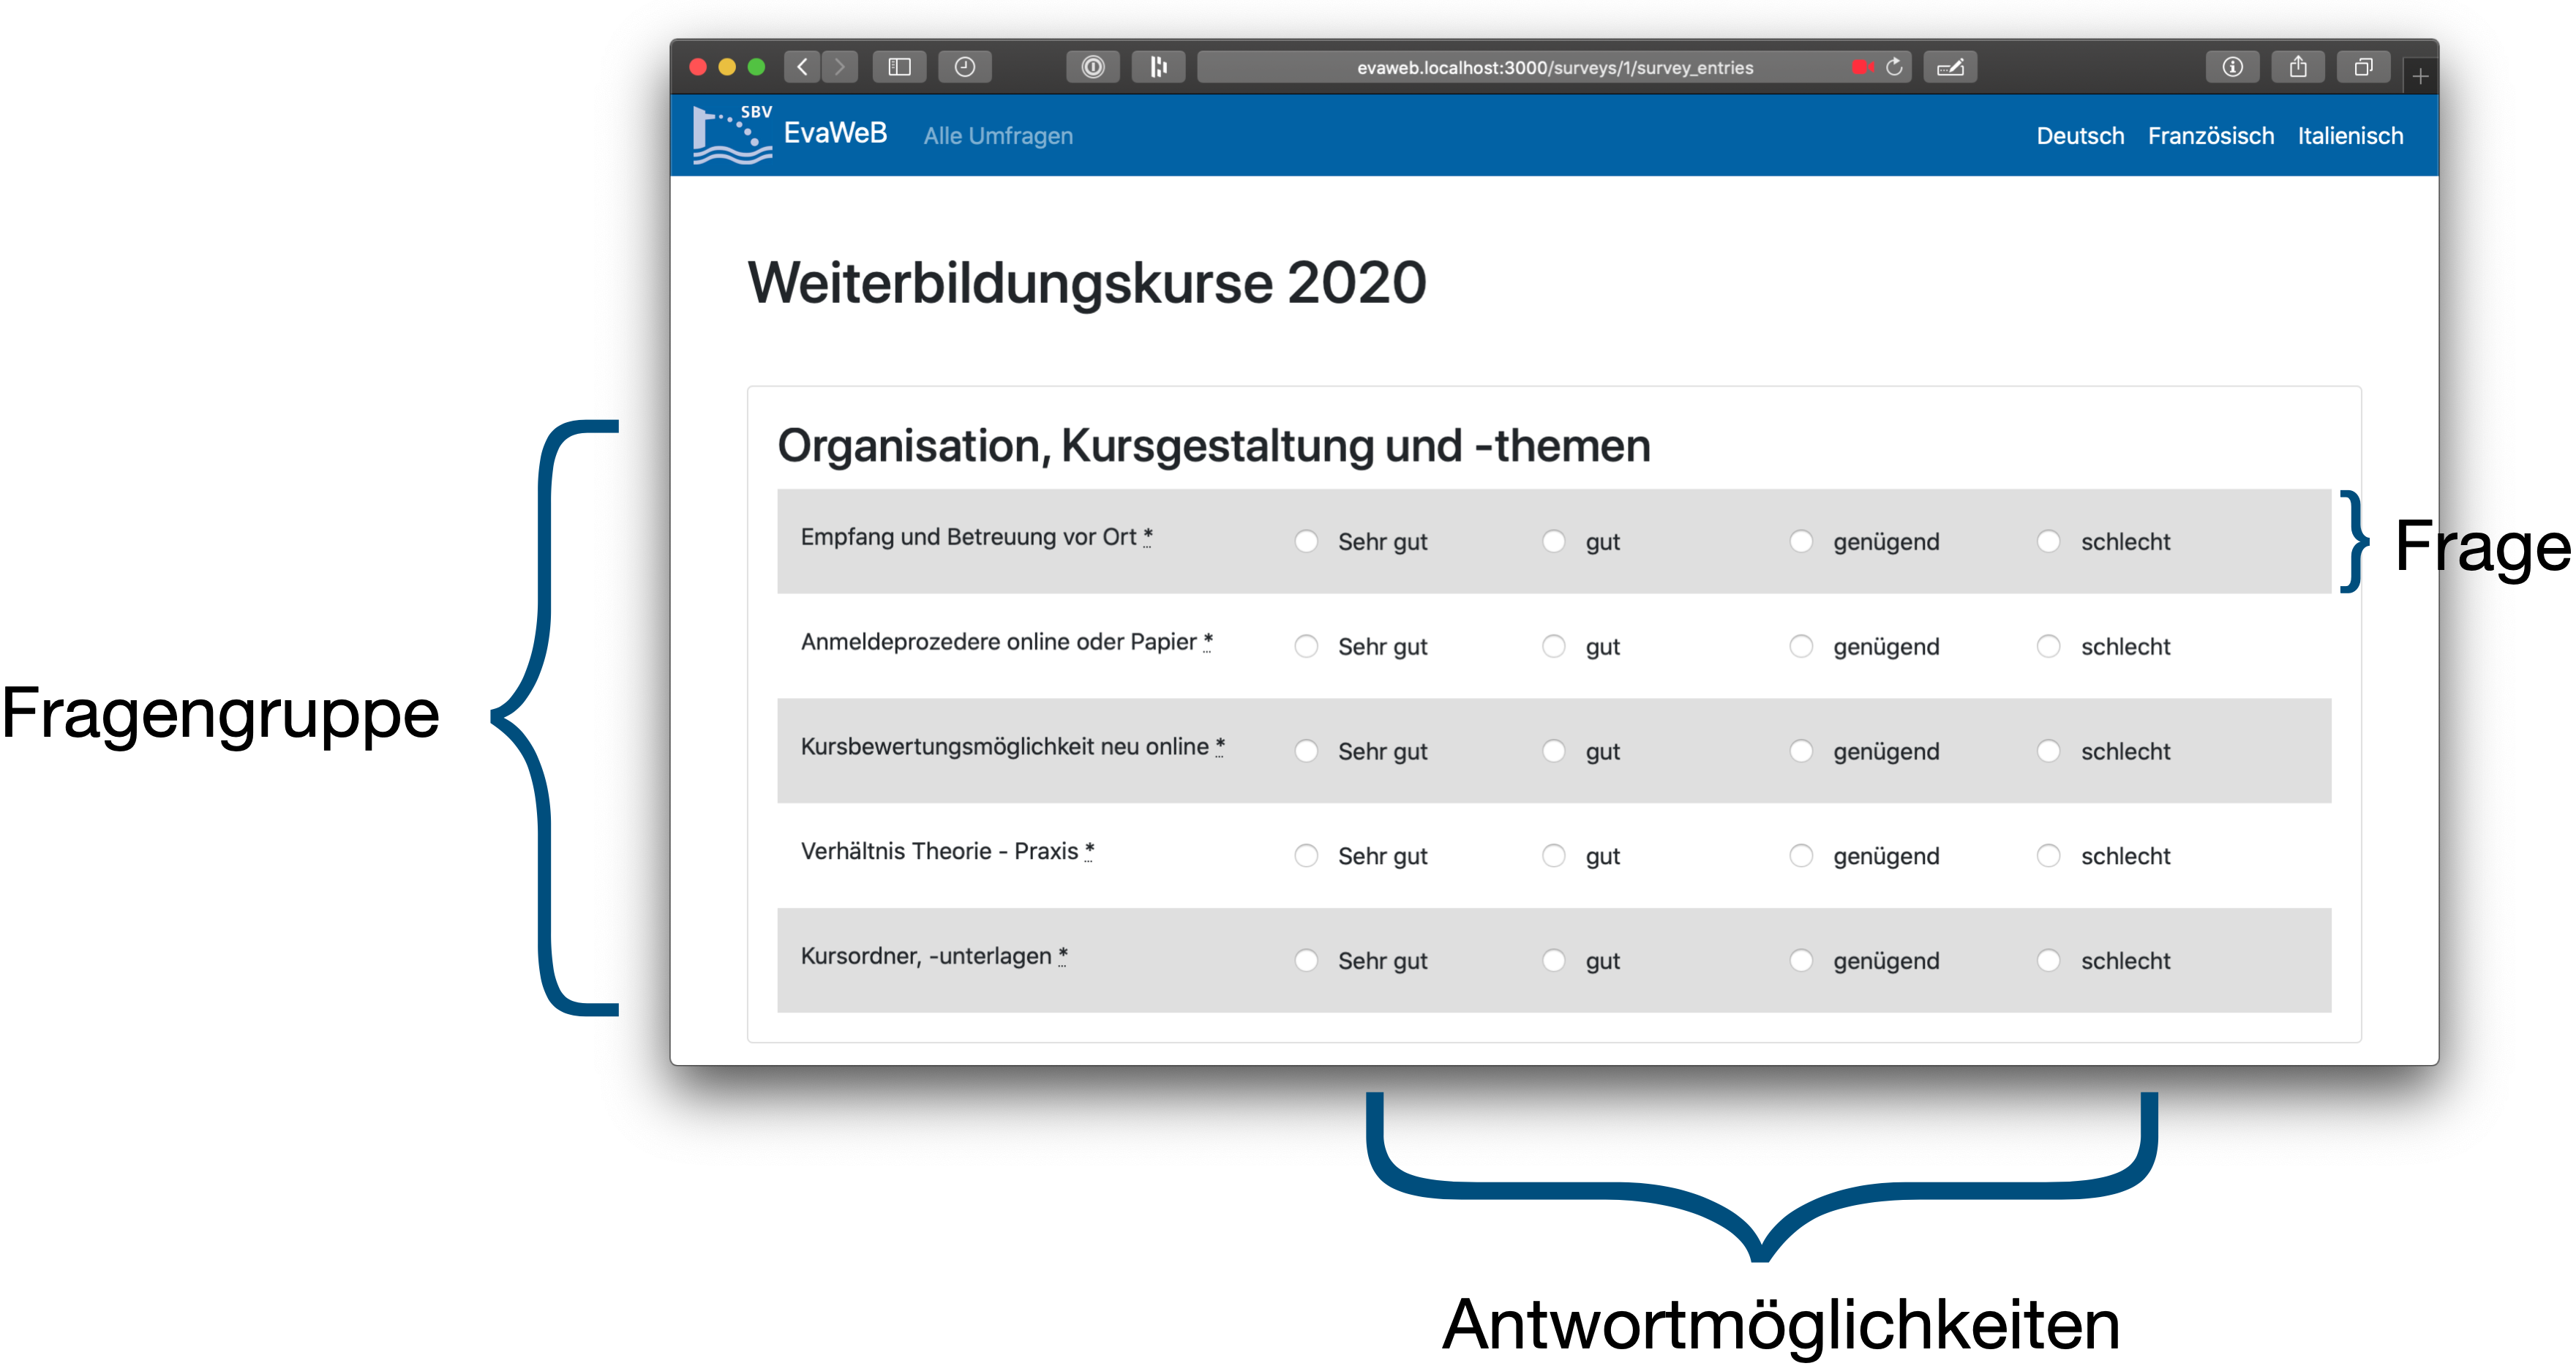
\includegraphics[width=\textwidth]{terminology.png}

\begin{enumerate}
    \item Umfrage
    \begin{enumerate}
        \item Eine Umfrage besitzt einen Titel und mehrere Fragengruppen
        \item 
            Eine Umfrage ist zeitlich begrenzt. 
            Das heisst, sie hat einen Start- und Endzeitpunkt, 
            zwischen denen die Umfrage aktiv ist und Antworten akzeptiert werden.
            Wenn man eine Umfrage anklickt, die nicht mehr aktiv ist, gibt es eine Fehlermeldung,
            dass die Umfrage nicht gefunden werden konnte.
    \end{enumerate}
    \item Fragengruppe
    \begin{enumerate}
        \item Jede Gruppe besteht aus einem Titel und mehreren Fragen
        \item Eine Fragengruppe ist einzigartig für jede Umfrage
        \item Eine Fragengruppe sollte zwingend Fragen beinhalten
    \end{enumerate}
    \item Frage
    \begin{enumerate}
        \item Eine Frage besteht aus einem Text/Frage und mehreren 
        Antwortmöglichkeiten
        \item Jede Frage innerhalb einer Fragengruppe muss aus denselben
        Antwortmölichkeiten bestehen, damit sie für die Auswertung gruppiert werden können.
    \end{enumerate}
    \item Antwortmöglichkeit
    \begin{enumerate}
        \item Eine Antwortmöglichkeit hat einen Text (bspw. "Sehr gut")
        \item Eine Antwortmöglichkeit kann von mehreren Fragen verwendet werden
    \end{enumerate}
\end{enumerate}

\pagebreak
\section{Dashboard}
Das Dashboard kann grundsätzlich nur von einem Administrator angesehen werden. 
Dementsprechend sollte man sich einloggen, bevor man das Dashboard aufruft.

\begin{flushleft}
Das Dashboard kann entweder auf der Umfrage selbst aufgerufen werden:
\\[0.2cm]
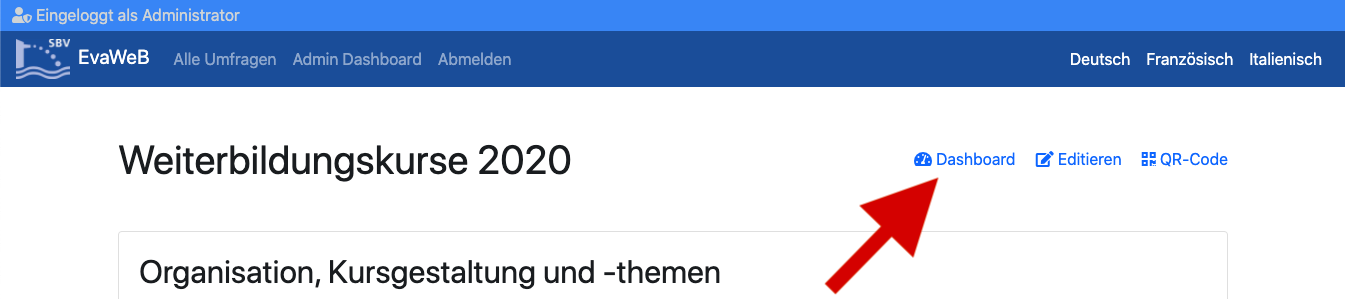
\includegraphics[width=\textwidth]{images/dashboard_link_beispiel_1.png}
\\[0.7cm]
Oder auch im Administrator-Tool auf der Umfragenansicht:
\\[0.2cm]
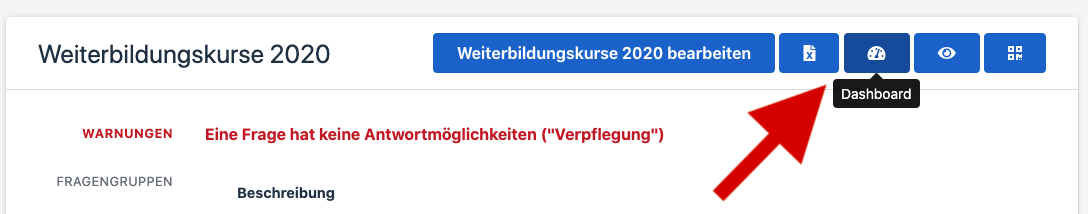
\includegraphics[width=\textwidth]{images/dashboard_link_beispiel_2.png}
\end{flushleft}

\subsection{Struktur}
Das Dashboard ist dabei folgendermassen strukturiert:

\inlineimage{images/survey.png}
Die Auswertung bei Umfragen, für die es noch keine Antworten gibt, wird nicht angezeigt, bzw. nur der Link mit QR-Code.


\pagebreak
\section{Umfragen}
Das Tool ist so ausgelegt, dass bei jeder Weiterbildung neue Umfragen für jeden Tag erstellt werden. 
Jede Umfrage hat einen Zeitrahmen, in der sie aktiv ist. 
Während diesem Zeitrahmen können die Teilnehmer die Umfrage öffnen und ausfüllen, sowie abschicken.
Jede Eingabe wird dann auf dem Dashboard live reflektiert.
Die Umfrage kann entweder über die Eingabe der URL oder über den QR-Code, welcher auf dem Dashboard der jeweiligen Umfrage
dargestellt wird, geöffnet werden. 

\pagebreak
\subsection{Flyer}
Solange man als Administrator eingeloggt ist, kann man für jede Umfrage einen kleinen Flyer generiert werden, 
auf dem der QR-Code und die URL ebenso aufgeführt sind. Dieser kann dann den Teilnehmern verteilt werden.
Dazu klickt man im Admin-Tool in der Umfrageübersicht auf das kleine QR-Code Symbol:
\\[0.2cm]
\inlineimage{images/dashboard_link_beispiel3.png}

\begin{flushleft}
Danach wird man weitergeleitet auf eine Vorschau des Flyers, welcher dann mit der
kleinen Druck-Knopf ausgedruckt werden kann:
\\[0.25cm]
\inlineimage{images/flyer.png}
\end{flushleft}{}

\pagebreak
\subsection{Export}
Nachdem eine Umfrage abgeschlossen wurde, kann man sie als Excel exportieren lassen, für die weitere Verarbeitung.
Dazu gibt es eine Schaltfläche im Admin-Tool in der Umfragenübersicht:
\\[0.2cm]
\inlineimage{images/excel_export.png}

\pagebreak
\section{Administrations-Tool}
\subsection{Login}
Unter \underline{https://evaweb-production.herokuapp.com/administrators/sign\_in}
kann man sich als Administrator einloggen.

\subsection{Administrations-Menü}
Nach dem Login kann man unter \underline{https://evaweb-production.herokuapp.com/admin}
in den Administrations-Teil einsteigen.
Auf der linken Seite erscheint das Administrations-Menü
\newline
\inlineimage{images/adminDashboard.png}
\\[.5cm]
Hier sind die 5 Datensätze aufgelistet. Ausserdem hat es einen Link auf die Startseite und einen um sich abzumelden.

\pagebreak
\subsubsection{Datensatz erstellen}
Mit einem Klick auf die Schaltfläche oben rechts wird ein neuer Datensatz erstellt.
\newline
\inlineimage{images/adminDashboardNeu.png}
\\[1.5cm]
Nachdem man alle Felder ausgefüllt hat kann man mit der Schaltfläche unten den Datensatz speichern.
\newline
\inlineimage{images/adminDashboardNeuSpeichern.png}

\subsubsection{Datensatz aktualisieren}
Um einen Datensatz zu aktualiseren kann man ihn in der Liste anklicken.
\newline
\inlineimage{images/adminDashboardListe.png}

\subsubsection{Fehler beim aktualisieren oder erstellen}
Falls beim erstellen oder aktualiseren eines Datensatzes ungültige oder unvollständige Angaben gemacht wurden, wird dies im oberen Bildschirm-Bereich angezeigt
\newline
\inlineimage{images/adminDashboardNeuFehler.png}

\pagebreak
\subsubsection{Eingabehilfe für Datums- und Zeitwerte}
Wenn ein Feld für ein Datumswert angeklickt wird öffnet sich die Eingabehilfe für Zeit- und Datumswerte.
\newline
\inlineimage{images/adminDashboardZeitPicker.png}

\subsection{Umfragen-Menü}
Auf der Hauptseite (https://evaweb-production.herokuapp.com/) erscheint eine neue Informationsleiste, wenn man als Administrator angemeldet ist.
\newline
Ausserdem erscheinen auf der normalen Menüleiste noch zwei weitere Schaltflächen.
\newline
\inlineimage{images/adminFrontendBar.png}

\renewcommand{\bibsection}{\section{Quellen}}
\bibliographystyle{plain}
% \bibliography{references}
\end{document}
